\documentclass[../../main]{subfiles}

\renewcommand\thesection{\arabic{section}}


\begin{document}

\section{Warm and Cool Lighting Control} \label{sec:}

It is required to expose the plants to the right amount of light, for their growth.
This part of the system tries to exactly do that. Right now we have chosen expose
the plant with \emph{warm} and \emph{cool} lights\footnote{full spectrum is preferred}.

\begin{center}
    {\begin{minipage} [c] {0.55\textwidth}

        Figure \ref{fig:warmLightImage}, shows the warm version of the LED, there
        will be a cool version similar to this. These LEDs are rated for 1W, and
        we need a driving circuit to drive these LEDs.

        We can simply \emph{low side switch} them using \emph{BC547}, if we could
        can limit the current. We can simply use a $68\si{k\ohm}$ resisters to
        limit the current, and can drive them like shown in the circuit digram
        shown in figure \ref{fig:clvlCtkLEDDriver}.

    \end{minipage}
    \hfill
    \begin{minipage} [c] {0.35\textwidth}
        \centering
        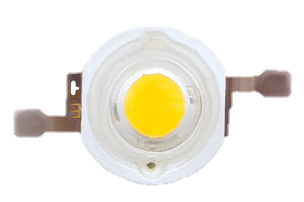
\includegraphics [
            max width = \IGXMaxWidth,
            max height = \IGXMaxHeight,
            \IGXDefaultOptionalArgs,
        ] {pics/1w_light.png}
        \captionof{figure} {
            Warm COB \emph{LED}.
            \label{fig:warmLightImage}
        }
    \end{minipage}\hfill}
\end{center}

\begin{center}
    {\begin{minipage} [c] {0.55\textwidth}
        The $68 \si{\ohm}$ will limit the current to:
        \begin{align}
            I &= 5 \si{V} / 68 \si{\ohm} \\
            &= 0.073 \si{A}
        \end{align}

        Which is well in-spec with the rating of \emph{BC547}.

        And also note that the base resistance is taken as $10 \si{k \ohm}$.

    \end{minipage}
    \hfill
    \begin{minipage} [c] {0.35\textwidth}
        \centering
        \includegraphics [
            max width = \IGXMaxWidth,
            max height = \IGXMaxHeight,
            \IGXDefaultOptionalArgs,
        ] {tikzpics/endClvlCtkLEDDriver.pdf}
        \captionof{figure} {Driving circuit for LEDs.}
        \label{fig:clvlCtkLEDDriver}
    \end{minipage}\hfill}
\end{center}

\alertImportant{
    Plants requires some part of the UV\footnote{UVA range, from $315-400$nm range.} light
    and full spectrum of the visible light to properly grow. Most of the greenhouse enclosures are
    good blockers of UV\footnote{Glass usually blocks $95\%$ of all the UV.}, it is required to
    expose the seedlings to UV light as well as the visible light. But right now we haven't done
    that, but it would be easy as adding just another light.
}

\begin{figure}
    \centering
    \includegraphics [
        max width = \IGXMaxWidth,
        max height = \IGXMaxHeight,
        \IGXDefaultOptionalArgs,
    ] {tikzpics/endAbsLightingControlSystem.pdf}
    \captionof{figure} {Interfacing of LEDs with \esp.}
    \label{fig:ledInterfacing}
\end{figure}

\alertNote{
    Trigger pin of \emph{LEDs} is connected to the \texttt{D18} and \texttt{D19} of the \esp as we can see
    from figure \ref{fig:ledInterfacing}.
}

\alertImportant{
    Right now, the \emph{LEDs} are triggered directly from the \esp itself. In the future
    all the \emph{actuator control} will be moved to the \emph{auxiliary system} with a separate
    control board\footnote{will be another shift register board.} and \esp will simply interface
    the board through couple of pins.
}
\end{document}
